\documentclass[../../tc_tp5_main.tex]{subfiles}

\begin{document}

%capitulo
\chapter{Sedra-Ghorab-Martin}

\section{Introducci\'on}

\subsection{Usos}

La celda Sedra-Ghorab-Martin implementa una funci\'on transferencia de orden 2 utilizando un solo op-amp, por lo que se dice que es una celda \textit{SAB} \textit{(single-amplifier-biquad)}. Se destaca por tener una baja sensibilidad del Q de los polos respecto a la ganancia de lazo abierto comparada con otras topolog\'ias (por ejemplo, la Sallen-Key analizada en el ejercicio 1). A cambio de esta ventaja, aumenta la sensibilidad respecto a los componentes pasivos.

En esta secci\'on se utiliza la metodolog\'ia descripta en la publicaci\'on \textit{Optimum Configurations for Single-Amplifier Biquadratic
Filters} de Adel S. Sedra, Mohamed A. Ghorab y Ken Martin para obtener un filtro pasabajos con la siguiente plantilla:
\begin{center}
\begin{tabular}{|c|c|}
\hline 
$f_a$ & 12.2KHz \\ 
\hline 
$f_p$ & 24.4KHz \\ 
\hline 
$A_p$ & 2dB \\ 
\hline 
$A_a$ & 40dB \\ 
\hline 
$\abs{Z_{in}(f)}$ & >50K$\Omega$ \\ 
\hline 
\end{tabular} 
\end{center}

Se analiza el solamente el circuito HPB ya que el LPB no fue utilizado.


\section{Obtenci\'on funcion transferencia con Cauer}

Se uiliz\'o la aproximaci\'on de Cauer. Vale la pena mencionar que \'esta tiene ceros sobre el eje imaginario, por lo que peque\~nas variaciones en los par\'ametros del circuito puedan llevar los ceros de un lado al otro del eje. Este fen\'omeno no afecta significativamene el m\'odulo de la transferencia, pero s\'i cambia el sentido del salto de 180$^\circ$ en la fase en $f_z$. 
Para obtener la funci\'on transferencia, se us\'o una plantilla m\'as restrictiva: $A_a$ = 41dB y $A_p$ = 1dB, y se uso una desnormalizaci\'on del 50\% entre $f_a$ y $f_p$. Con estas consideraciones se obtuvo la funci\'on transferencia del filtro y se divisi\'o en etapas:


Filtro total:
\begin{equation}
H(s) = \frac{3.43\cdot s^4 + 2.73 \cdot 10^{10}\cdot s^2+ 3.01\cdot 10^{19} }{4.075 \cdot s^4 + 1.223\cdot 10^{06}\cdot  s^3 + 3.077\cdot 10^{11}\cdot s^2 + 2.549\cdot 10^{16}\cdot s + 3.67\cdot {21}}
\end{equation}

\begin{figure}[H]	%H y pz filtro
	\centering
	\begin{subfigure}[t]{0.7\textwidth}
		\centering
		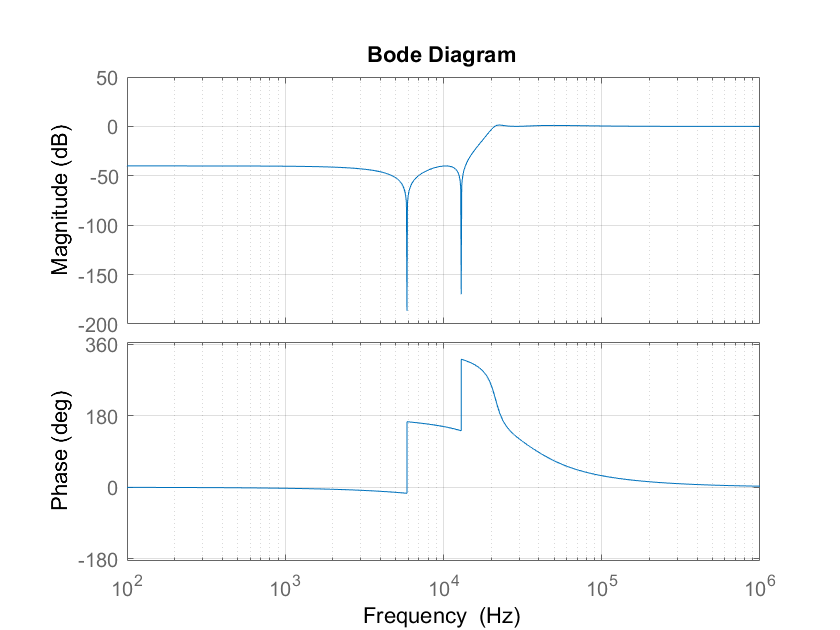
\includegraphics[width=\textwidth]{imagenes/bode_total_calculo_pablo.png}
		\caption{Funci\'on transferencia del filtro}
		\label{fig:ej3_H_ideal}
	\end{subfigure}%
	\hfill%%
	\begin{subfigure}[t]{0.7\textwidth}
		\centering
		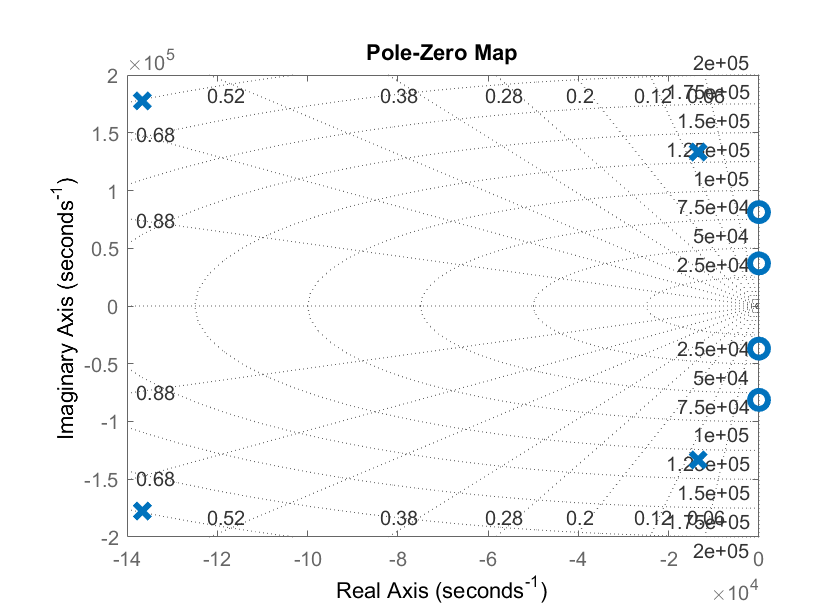
\includegraphics[width=\textwidth]{imagenes/pz_total.png}
		\caption{Diagrama polos y ceros del filtro}
		\label{fig:ej3_pz_total}
	\end{subfigure}
\end{figure}

Se dividieron los polos y ceros en dos etapas:

Primera etapa:
\begin{itemize}
	\item $f_z$ = 12.9 KHz
	\item $f_0$ = 21.3 KHz
	\item Q = 4.67
	\item Gain = -0.5dB
\end{itemize}

\begin{equation}
H_1(s) = \frac{4.69\cdot s^2+3.1\cdot 10^{10}}{4.97\cdot s^2+1.34\cdot 10^5\cdot s + 8.92\cdot 10^{10}}
\end{equation}

\begin{figure}[H]	%H y pz etapa 1
	\centering
	\begin{subfigure}[t]{0.7\textwidth}
		\centering
		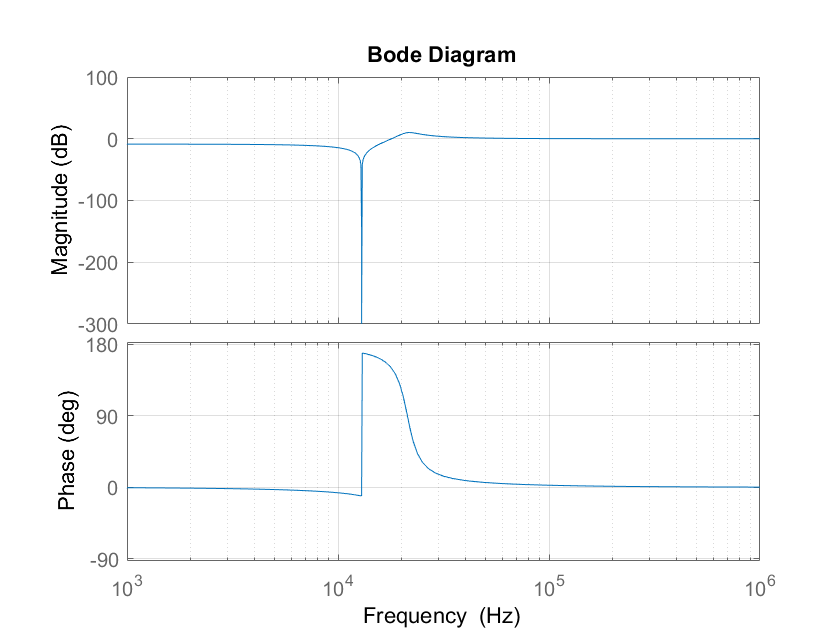
\includegraphics[width=\textwidth]{imagenes/bode_etapa_1_calculo_pablo.png}
		\caption{Funci\'on transferencia de la etapa 1}
		\label{fig:ej3_H1_ideal}
	\end{subfigure}%
	\hfill%%
	\begin{subfigure}[t]{0.7\textwidth}
		\centering
		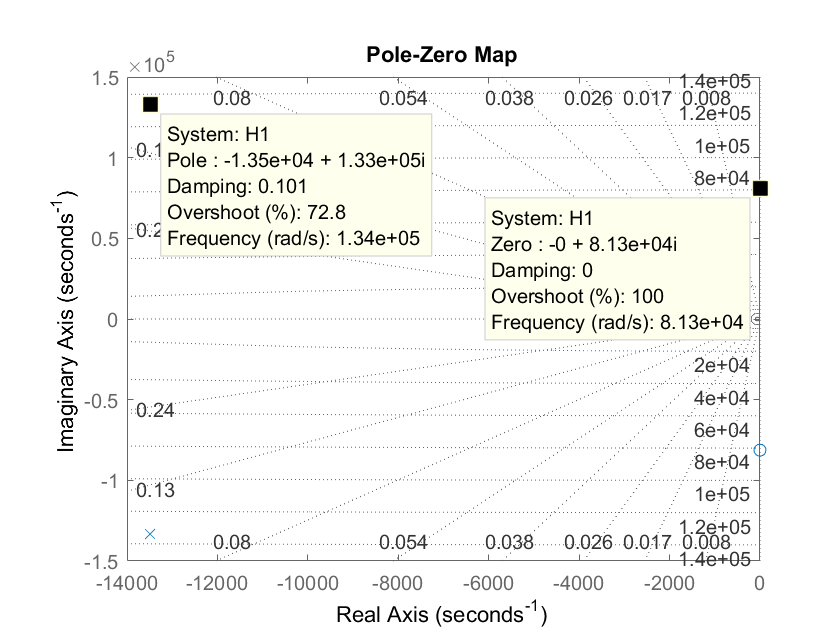
\includegraphics[width=\textwidth]{imagenes/pz_etapa_1.png}
		\caption{Diagrama polos y ceros de la etapa 1}
		\label{fig:ej3_pz_etapa_1}
	\end{subfigure}
\end{figure}


Segunda etapa
\begin{itemize}
	\item $f_0$ = 5.9KHz 
	\item $f_p$ = 35.6 KHz
	\item Q = 0.82
	\item Gain = -1dB
\end{itemize}

\begin{equation}
H_2(s)\frac{0.73\cdot s^2+9.96\cdot 10^{8}}{0.82\cdot s^2+2.24\cdot 10^5\cdot s + 4.12\cdot 10^{10}}
\end{equation}

\begin{figure}[H]	%H y pz etapa 2
	\centering
	\begin{subfigure}[t]{0.7\textwidth}
		\centering
		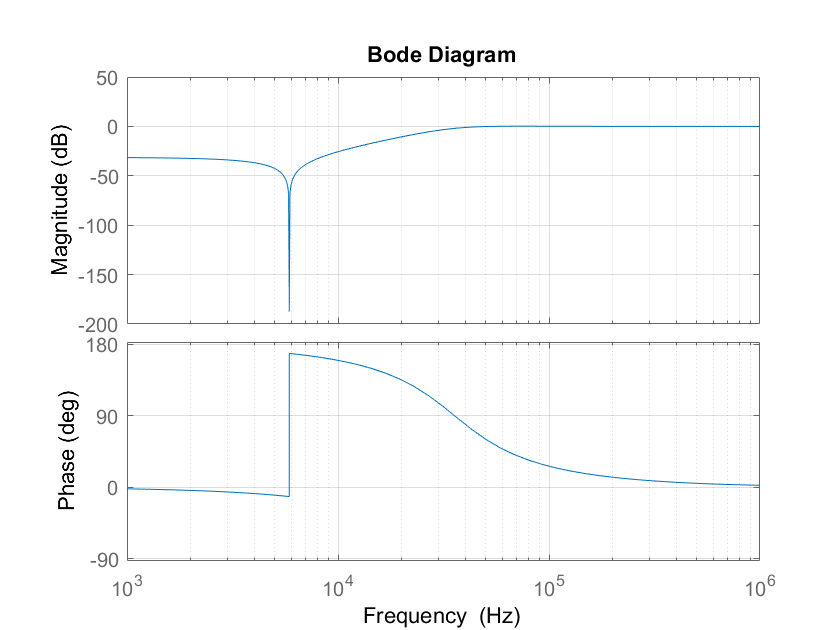
\includegraphics[width=\textwidth]{imagenes/bode_etapa_2_calculo_pablo.png}
		\caption{Funci\'on transferencia de la segunda etapa}
		\label{fig:ej3_H2_ideal}
	\end{subfigure}%
	\hfill%%
	\begin{subfigure}[t]{0.7\textwidth}
		\centering
		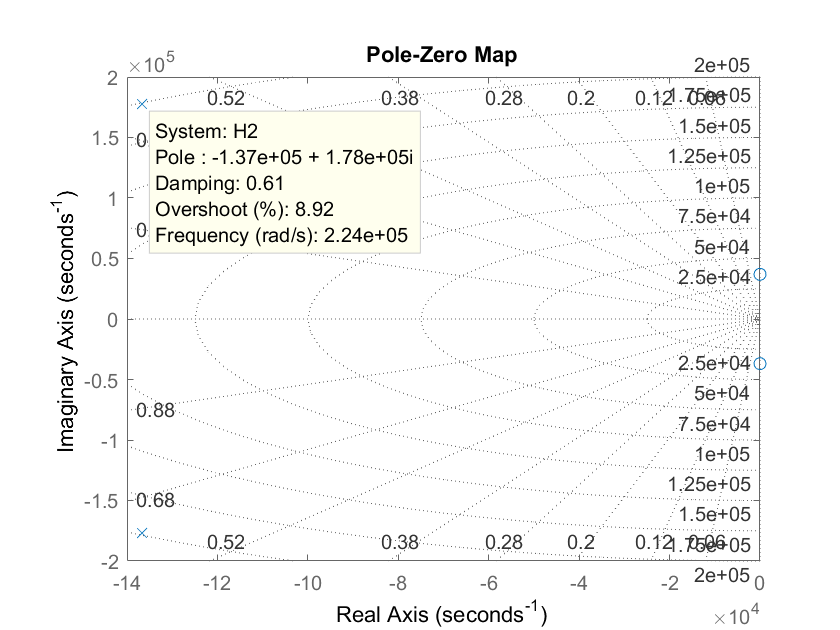
\includegraphics[width=\textwidth]{imagenes/pz_etapa_2.png}
		\caption{Diagrama polos y ceros de la segunda etapa}
		\label{fig:ej3_pz_etapa_2}
	\end{subfigure}
\end{figure}


Dado que las dos etapas son filtros high-pass notch, se utiliz\'o el circuito HPB dos veces (figura \ref{HPB})

\begin{figure}[H]
\centering
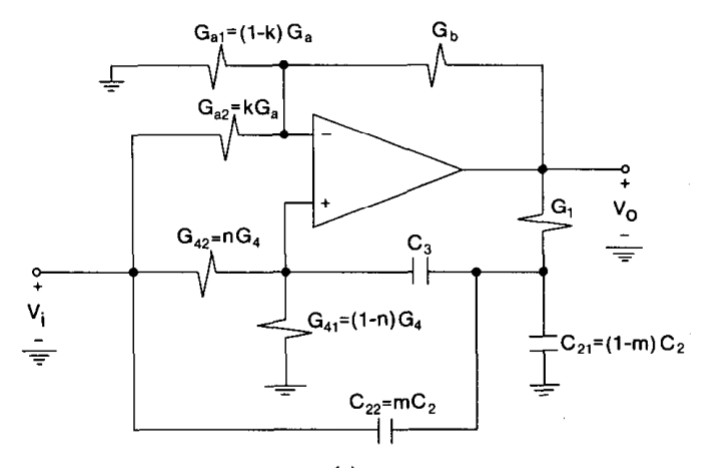
\includegraphics[scale=1]{imagenes/HPB.png}
\caption{Circuito HPB}
\label{HPB}
\end{figure}

\section{Elecci\'on de componentes}

Se sigui\'o el proceso de selecci\'on de componentes detallado en el paper, eligiendo  $Q_0 = \frac{Q}{3}$ para la primer etapa y $Q_0 = \frac{Q}{5}$ para la segunda, y $\frac{1}{G_b} = 1K\Omega$.


\begin{table}[H]
\centering
\begin{tabular}{l|ll}
\hline
    & Etapa1   & Etapa2   \\
    \hline
Ra1 & 6,37E-05 & 2,35E+02 \\
Ra2 & 7,18E-05 & 5,88E+03 \\
Ra  & 1,35E-04 & 2,26E+02 \\
Rb  & 1,00E-03 & 1,00E+03 \\
R1  & 2,17E-03 & 1,67E+03 \\
R41 & 1,42E-04 & 5,21E+02 \\
R42 & 8,29E-05 & 1,39E+04 \\
R4  & 2,25E-04 & 5,02E+02 \\
C21 & 5,60E-09 & 3,87E-09 \\
C22 & 4,67E-09 & 1,00E-09 \\
C2  & 1,03E-08 & 4,87E-09 \\
C3  & 5,23E-09 & 4,87E-09 \\
\hline
\end{tabular}
\end{table}


\begin{table}[H]
\centering
\begin{tabular}{l|llll}
\hline
Sensibilidades & $S_X^G$   & $S_X^Q$   & $S_X^W0$  & $S_X^Wz$  \\
\hline
Ra1            & -0.34 & 0.60  & 0.00  & -0.24 \\
Ra2            & 0.04  & 0.66  & 0.00  & 0.74  \\
Rb            & 0.29  & -1.26 & 0.00  & -0.50 \\
R41            & 0.00  & -0.48 & -0.32 & 0.76  \\
R42            & 0.00  & -0.28 & -0.18 & -1.26 \\
R1            & 0.00  & 0.76  & -0.50 & -0.50 \\
C3            & 0.00  & -0.63 & -0.50 & -0.50 \\
C21            & 0.15  & 0.56  & -0.45 & -0.52 \\
C22           & -0.15 & 0.07  & -0.05 & 0.02 \\
\hline
\end{tabular}
\end{table}



\subsection{Uso y ubicaci\'on del preset}
Con los valores elegidos y con tolerancias del 10\% para los capacitores y 1\% para las resistencias (las m\'inimas disponibles en el pa\~nol), el an\'alisis de Montecarlo indica que hay posibilidad de que el circuito no cumpla con la plantilla (ver figura \ref{fig:ej3_mc_filtro_mag}. Para solucionar esto, se utliz\'o un preset. Se eligi\'o ubicarlo en $R_b$ ya que es el componente qe tiene mas sensibilidad con Q, y adem\'as tiene sensibilidad cero respecto a $f_0$, por lo que permite modificar el Q del polo sin cambiar su frecuencia de corte.



\begin{figure}[H]	%montecarlo
	\centering
	\begin{subfigure}[t]{0.7\textwidth}
		\centering
		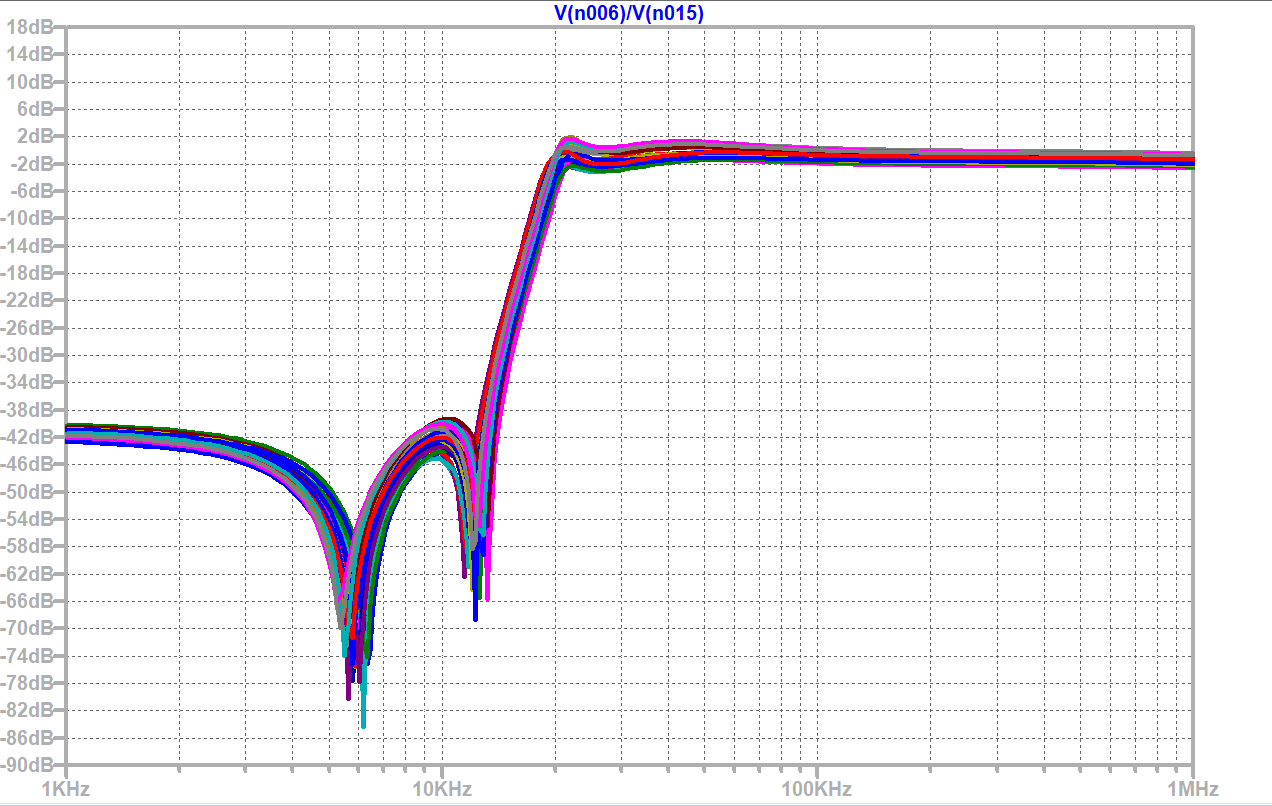
\includegraphics[width=\textwidth]{imagenes/montecarlo_total.png}
		\caption{Magnitud. Notar que en la banda pasante supera los 2dB y tambi\'en est\'a por debajo de los -2dB.}
		\label{fig:ej3_mc_filtro_mag}
	\end{subfigure}\\
	\begin{subfigure}[t]{0.7\textwidth}
		\centering
		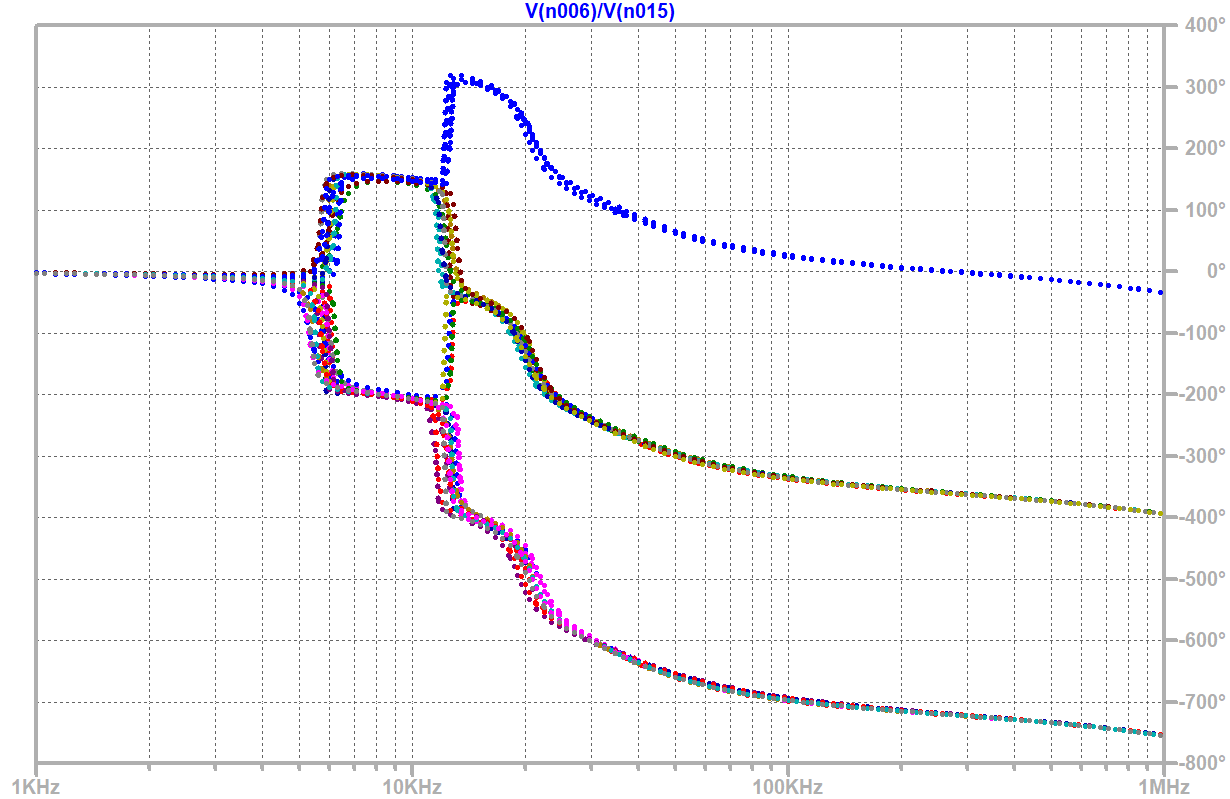
\includegraphics[width=\textwidth]{imagenes/montecarlo_total_fase.png}
		\caption{Fase}
		\label{fig:ej3_mc_filtro_fase}
	\end{subfigure}	
	\caption{An\'alisis de montecarlo del filtro}
\end{figure}


\subsection{Uso de buffers}

Se utiliz\'o un buffer en la entrada del circuito ya que la impedancia de entrada tiene valores cercanos a cero entre la frecuencia de atenuaci\'on y de paso (figura \ref{fig:ej3_zin_1}). Se agreg\'o otro buffer entre las etapas ya que la impedancia de salida de la etapa 1 es comparable con la de entrada de la etapa 2 (figuras \ref{fig:ej3_zin_2} y \ref{fig:ej3_zout_1}). Por ejemplo, a 20KHz, la impedancia de entrada de la segunda etapa es cercana a los 3.6$\Omega$ y la de salida de la primera es cercana a los 800$\Omega$. No se utiliz\'o un buffer en la salida del filtro ya que se consider\'o que una impedancia de salida menor a 75$\Omega$ era aceptable.





\begin{figure}[H]	%Zin
	\centering
	\begin{subfigure}[t]{\textwidth}
		\centering
		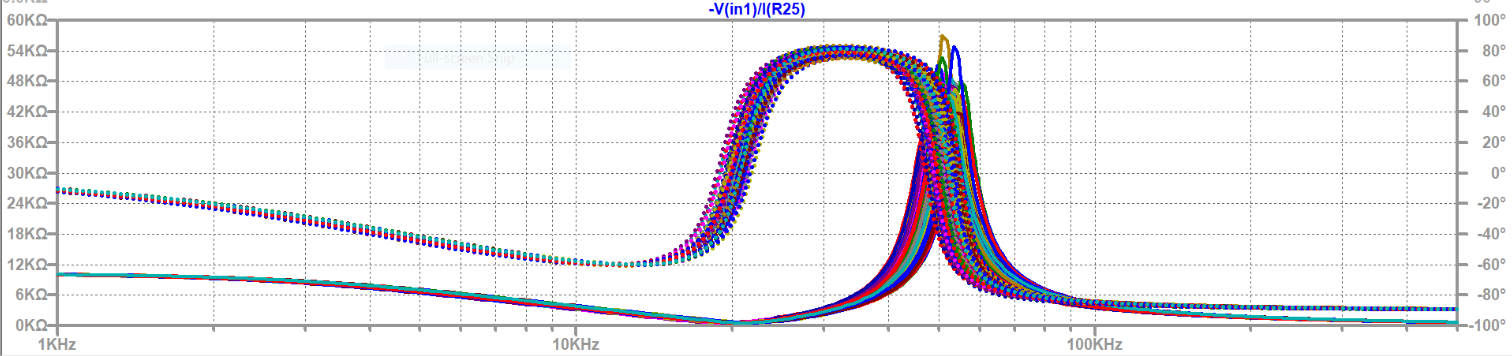
\includegraphics[width=\textwidth]{imagenes/zin_1.png}
		\caption{Etapa 1}
		\label{fig:ej3_zin_1}
	\end{subfigure}\\
	\begin{subfigure}[t]{\textwidth}
		\centering
		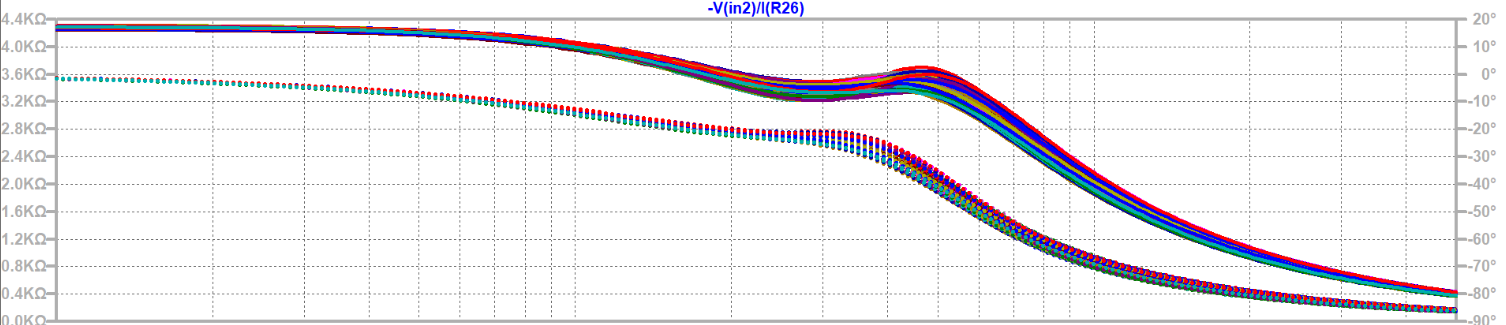
\includegraphics[width=\textwidth]{imagenes/zin_2.png}
		\caption{Etapa 2}
		\label{fig:ej3_zin_2}
	\end{subfigure}	
	\caption{Impedancias de entrada sin buffer}
\end{figure}

\begin{figure}[H]	%Zout
	\centering
	\begin{subfigure}[t]{\textwidth}
		\centering
		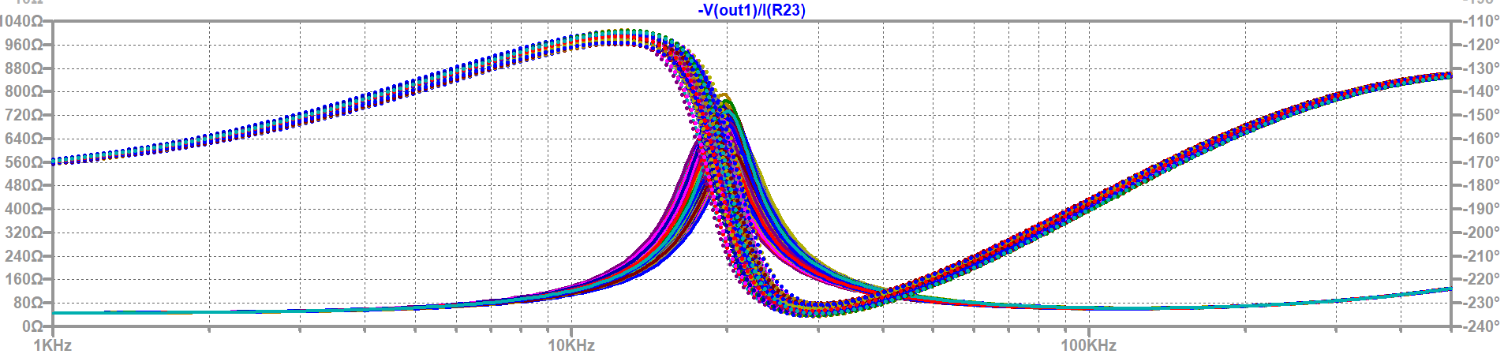
\includegraphics[width=\textwidth]{imagenes/zout_1.png}
		\caption{Etapa 1}
		\label{fig:ej3_zout_1}
	\end{subfigure}\\
	\begin{subfigure}[t]{\textwidth}
		\centering
		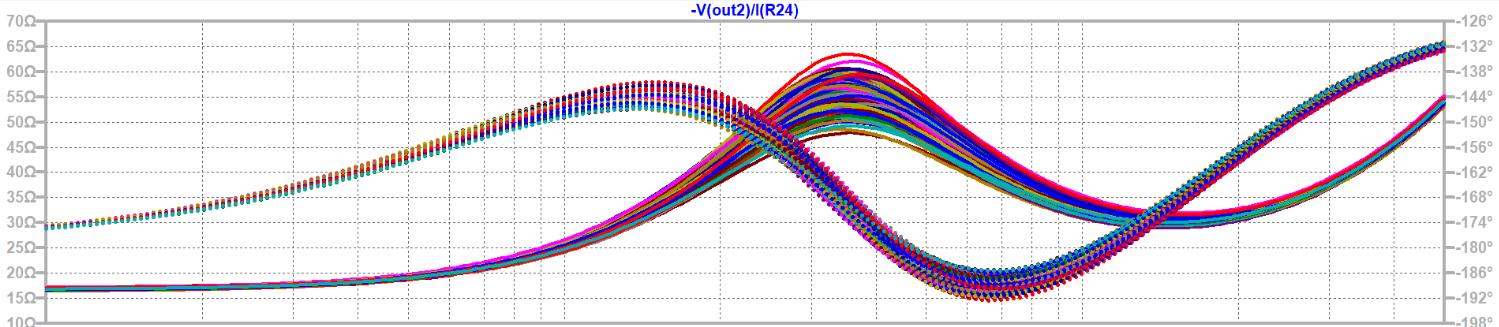
\includegraphics[width=\textwidth]{imagenes/zout_2.png}
		\caption{Etapa 2}
		\label{fig:ej3_zout_2}
	\end{subfigure}	
	\caption{Impedancias de salida sin buffer}
\end{figure}



\section{Mediciones}

Se realizaron mediciones de la respuesta en frecuencia de cada etapa por separado y en conexi\'on en cascada formando el filtro. Para esto no se utiliz\'o un osciloscopio, sino el \textit{Analog Discovery}, ya que puede recorrer todo el espectro a mayor velocidad, y esto permite ver en tiempo real como se modifica el circuito al cambiar la variable de ajuste. Luego de ser calibrado, el filtro cumple plantilla. Como se mencion\'o anteriormente, debido a un cambio en el semiplano en donde se encuentran los ceros, el salto de fase de 180$^\circ$ en $f_z$ se produce en el diferentes sentidos. 



\begin{figure}[H]
	\centering
	\begin{subfigure}[t]{0.8\textwidth}
		\centering
		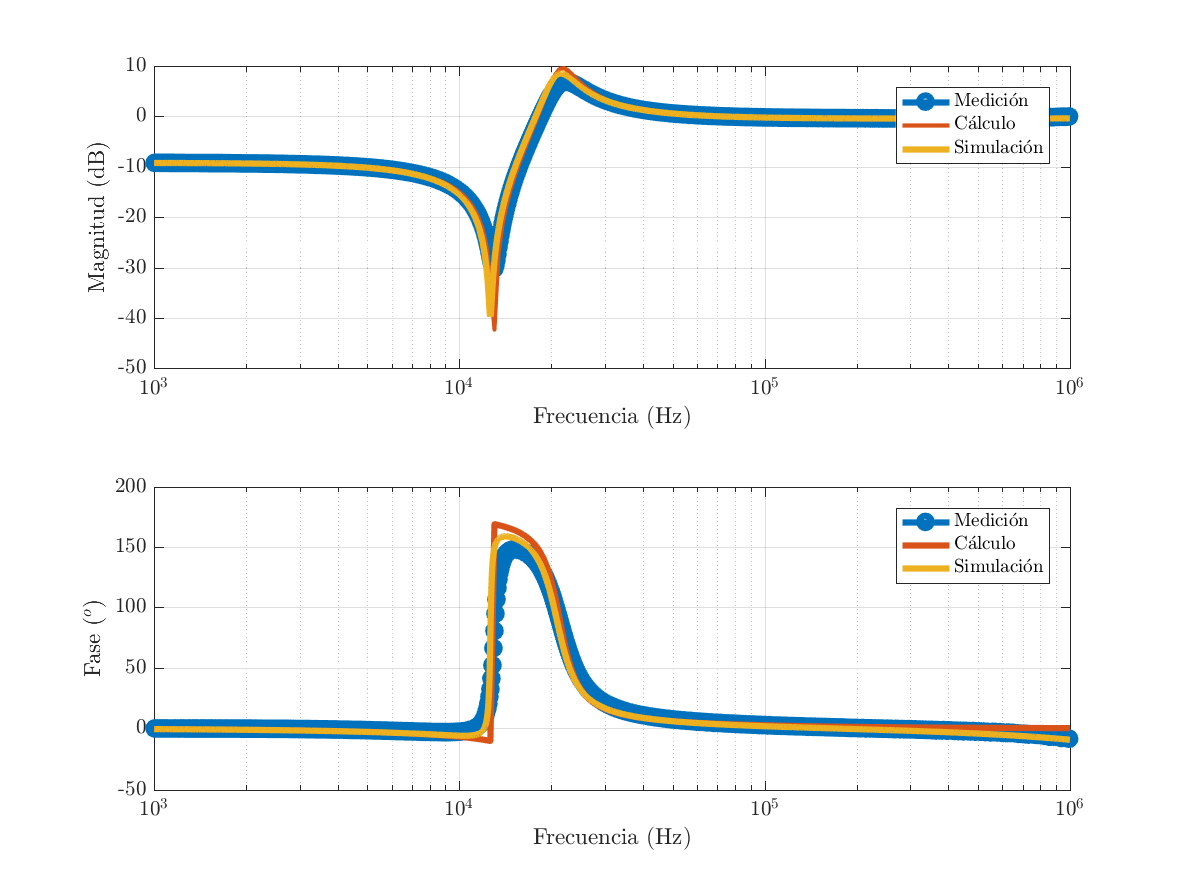
\includegraphics[width=\textwidth]{imagenes/etapa_1_bode.png}
		\caption{Etapa 1}
		\label{fig:ej3_bode_etapa_1}
	\end{subfigure}
\end{figure}
\begin{figure}[H]
\ContinuedFloat	
	\centering
	\begin{subfigure}[t]{0.8\textwidth}
		\centering
		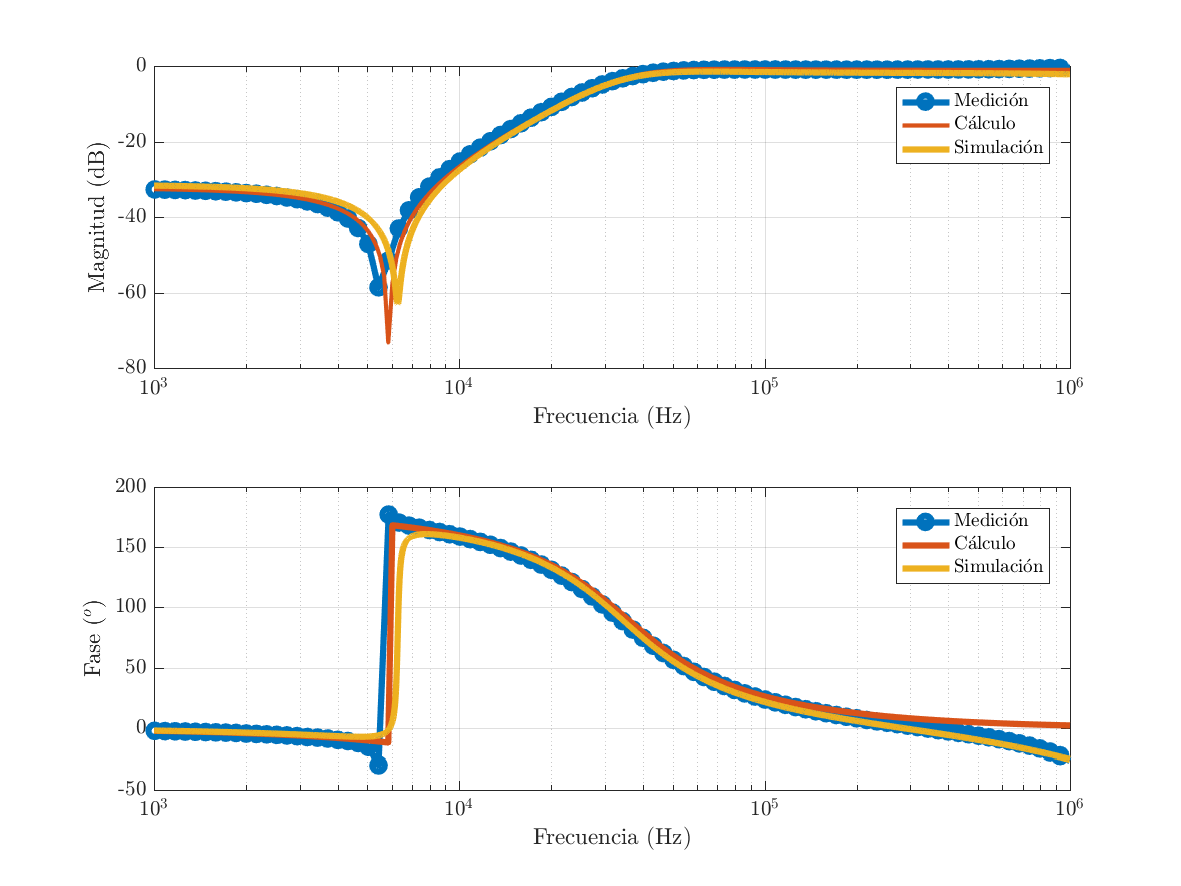
\includegraphics[width=\textwidth]{imagenes/etapa_2_bode.png}
		\caption{Etapa 2}
		\label{fig:ej3_bode_etapa_2}
	\end{subfigure}
\end{figure}
\begin{figure}[H]
\ContinuedFloat	
	\centering
	\begin{subfigure}[t]{0.8\textwidth}
		\centering
		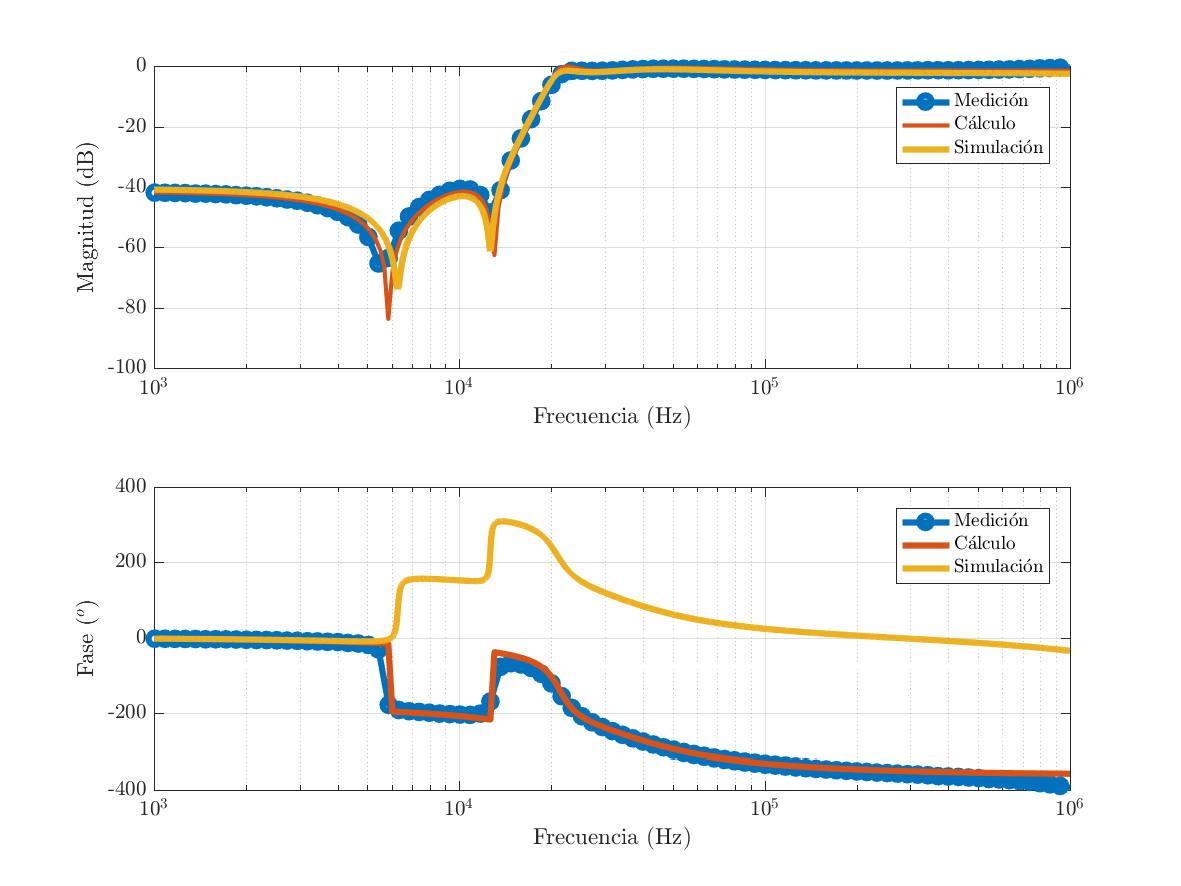
\includegraphics[width=\textwidth]{imagenes/total_bode.png}
		\caption{Filtro}
		\label{fig:ej3_bode_etapa_3}
	\end{subfigure}	
	\caption{Respuesta en frecuencia simulada, medida y calculada.}
\end{figure}








\section{Estabilidad}
Asumiendo que las etapas no se cargan entre s\'i, la  conexi\'on en cascada no modifica a los ceros de la funci\'on transferencia de las etapas como por ejemplo lo hace una conexi\'on en la que se agrega un lazo de realimentaci\'on, por lo que si ambas etapas son estables, el filtro es estable. Sin embargo, en este an\'alisis se desprecian los efectos de los buffers a la entrada de las celdas, los cuales pueden desestabilizar al circuito. 
Se hizo un an\'alisis de estabilidad de cada etapa considerando su margen de fase, pero este resulto incorrecto (posiblemente por un error de cuentas). Se lo describe en el anexo.

Una vez medida la respuesta en frecuencia, se pusieron en repetidas veces tanto una se\~nal cuadrada como una se\~nal senoidal de  frecuencias del orden de los 10MHz para intentar que el filtro oscile pero no se consigui\'o. 

\section{Anexo}

\subsection{Transformaci\'on complementaria: relaci\'on entre celda HPB y Deliyannis}

\begin{figure}[H]	%complementary transformation
	\centering
	\begin{subfigure}[t]{0.35\textwidth}
		\centering
		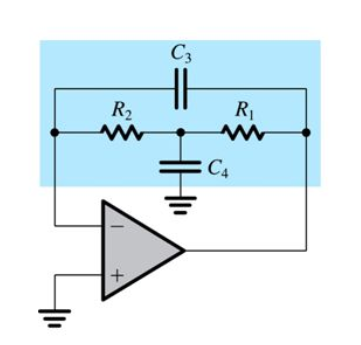
\includegraphics[width=0.8\textwidth]{imagenes/comp_trans_before.png}
		\caption{Estructura de feedback original}
		\label{fig:ej3_comp_trans_before}
	\end{subfigure}%
	\hfill
	\begin{subfigure}[t]{0.3\textwidth}
		\centering
		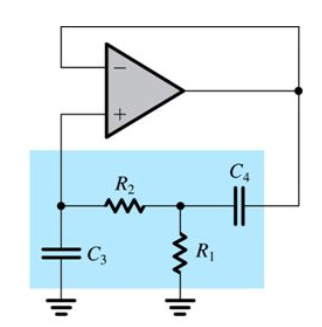
\includegraphics[width=\textwidth]{imagenes/comp_trans_after.png}
		\caption{Estructura de feedback luego de la transformacion complementaria}
		\label{fig:ej3_comp_trans_after}
	\end{subfigure}%
	\hfill
	\begin{subfigure}[t]{0.3\textwidth}
		\centering
		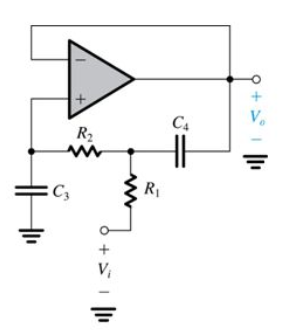
\includegraphics[width=\textwidth]{imagenes/comp_trans_signal.png}
		\caption{Circuito pasa bajos implementado con la estructura del circuito de la figura \ref{fig:ej3_comp_trans_after}}
		\label{fig:ej3_comp_trans_signal}
	\end{subfigure}	
	\caption{}
\end{figure}


La estructura de feedback de la celda HPB propuesta parte de aplicar la transformaci\'on complementaria a la estructura de feedback del circuito Deliyannis (figura \ref{fig:ej3_feedback_structure})


\begin{figure}[H]	%feedback structure
	\centering
	\begin{subfigure}[t]{0.47\textwidth}
		\centering
		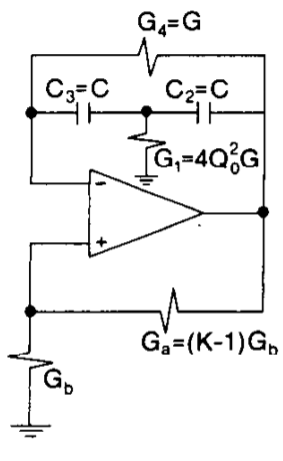
\includegraphics[width=0.6\textwidth]{imagenes/Deliyannis_feedback_structure.png}
		\caption{Estructura de feedback del circuito Deliyannis}
		\label{fig:ej3_feedback_structure_deliyannis}
	\end{subfigure}%
	\hfill
	\begin{subfigure}[t]{0.47\textwidth}
		\centering
		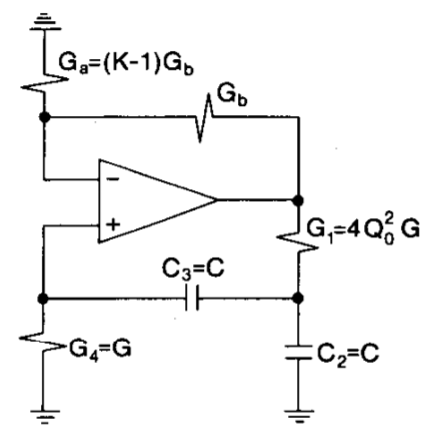
\includegraphics[width=\textwidth]{imagenes/sedra_HPB_feedback_structure.png}
		\caption{Estructura de feedback del high-pass biquad. Se obtiene aplicando las transformaciones complementarias.}
		\label{fig:ej3_feedback_structure_hpb}
	\end{subfigure}	
	\caption{}
	\label{fig:ej3_feedback_structure}
\end{figure}



\subsection{Transferencia con polo dominante por feedback}

Se muestra a continuaci\'on el desarrollo realizado para intentar obtener la funci\'on transferencia mediante el uso de diagramas de flujo de se\~nal y feedback teniendo en cuenta el polo dominante del op-amp. La ventaja de este m\'etodo de resoluci\'on es que se puede obtener r\'apidamente el loop-gain $L(s)$ del circuito y hacer un analisis de margen de fase para anlizar la estabilidad. Al reemplazar la H(s) obtenida con los valores de una de las dos celdas, la respuestas en frecuencia no coinciden, lo que lleva a concluir que hay un error de c\'alculo.

\begin{equation}
	V_0 = (V^+ - V^-)\cdot A_{vol}
\end{equation}
Nodo $V^-$:
\begin{equation}
	(V_i-V^-)\cdot G_{a2} + (V_0 - V^-)\cdot G_b - V^-  G_{a1} = 0
\end{equation}
\begin{equation}	
	V^- = V_i \cdot \frac{G_{a2}}{G_a G_b} + V_0\cdot \frac{G_b}{G_a+G_b}
\end{equation}
Si $K_1 = \frac{G_{a2}}{G_a G_b}$ y $K_2 = \frac{G_b}{G_a+G_b}$:
\begin{equation}
	V^-=K_1\cdot V_i + K_2 \cdot V_0
\end{equation}
Nodo $V^+$:
\begin{equation}
(V_0-V_A)G_1+(V^+-V_A)sC_3+(V_i-V_A)sC{22} = V_AsC_{21}
\end{equation}
\begin{equation}
V^+=V_i\frac{G_{42}}{G_4+C_2}+V_A\frac{sC_3}{G_4+sC_2}
\end{equation}
Nodo $V_A$:
\begin{equation}
(V_0-V_a)G_1+(V^+-V_A)sC_3+(V_i-V_A)sC{22}=sC_{21}V_A
\end{equation}
\begin{equation}
V_A = \frac{1}{sC_2+sC_3+G_1}\cdot(V_0G_1+V^+sC_3+V_1sC{22})
\end{equation}
Uniendo la expresi\'on de $V_A$ y de $V^+$ y con $M=\frac{sC_3}{(G_4+sC_2)(sC_2+sC_3+G_1)}$

\begin{equation}
V^+=V_i\frac{G_{42}}{G_4+sC_2}+V_0G_1\cdot M+V^+sC_3\cdot M + V_i sC_{22}\cdot M
\end{equation}
\begin{equation}
V^+=\frac{\frac{G_{42}}{G_4+C_2}+sC_{22}\cdot M}{1-sC_3\cdot M} \cdot Vi + \frac{G_1\cdot M}{1-sC_3\cdot M} \cdot V_0
\end{equation}
Con $K_3 = \frac{\frac{G_{42}}{G_4+C_2}+sC_{22}\cdot M}{1-sC_3\cdot M}$ y $K_4 = \frac{G_1\cdot M}{1-sC_3\cdot M}$:
\begin{equation}
V^+=K_3\cdot V_i+K_4\cdot V_0
\end{equation}



\begin{figure}[H]	%SFG para H
	\centering
	\begin{subfigure}[t]{0.8\textwidth}
		\centering
		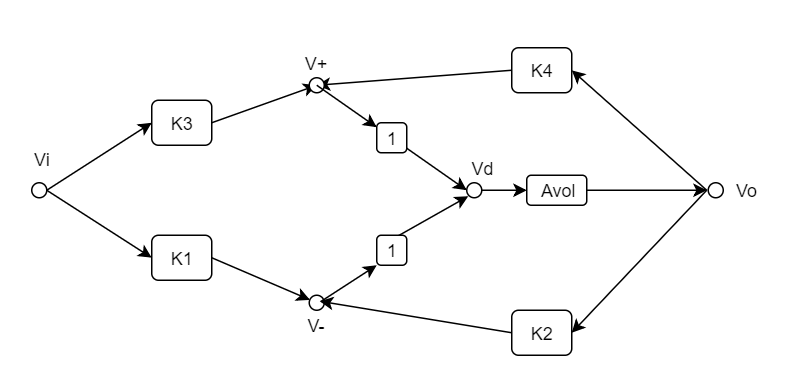
\includegraphics[width=0.8\textwidth]{imagenes/SFG1.png}
		\caption{Diagrama de flujo de se\~nal del high-pass notch.}
		\label{fig:ej3_SFG1}
	\end{subfigure}%
	\\
	\begin{subfigure}[t]{0.6\textwidth}
		\centering
		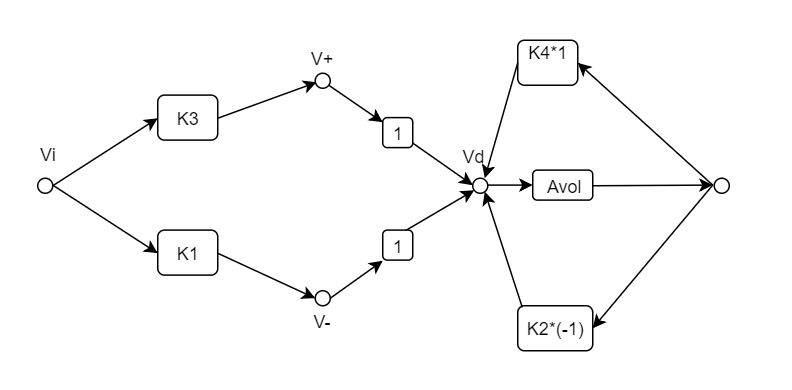
\includegraphics[width=\textwidth]{imagenes/SFG2.png}
		\caption{}
		\label{fig:ej3_SFG2}
	\end{subfigure}%
	\\
	\begin{subfigure}[t]{0.6\textwidth}
		\centering
		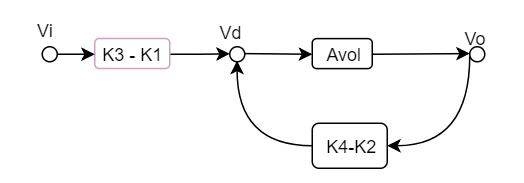
\includegraphics[width=\textwidth]{imagenes/SFG3.png}
		\caption{Feedback de la celda high-pass notch}
		\label{fig:ej3_SFG3_feedback}
	\end{subfigure}	
	\caption{}
\end{figure}



De la figura \ref{fig:ej3_SFG3_feedback} se obtiene la transferencia del filtro y el loop-gain L(s):
\begin{equation}
	H(s) = (K_3-K_1)\cdot \frac{A_{vol}}{1+(K_2-K_4)A_{vol}} \approx \frac{K_3-K_1}{K_2-K_4}	
\end{equation}
\begin{equation}
	L(s) = A_{vol}(K_3-K_1)
\end{equation}

\end{document}
